\documentclass{article}
\usepackage{graphicx,fancyhdr,amsmath,amssymb,amsthm,subfig,url,hyperref}
\usepackage[margin=1in]{geometry}
\usepackage{enumerate}
% \usepackage{algorithms}
\usepackage{bookmark}
\usepackage{tikz}
% \usetikzlibrary{arrows}
\usetikzlibrary{arrows.meta}
\usetikzlibrary{quotes}
\usepackage{extarrows}
\usepackage{clrscode3e}

%----------------------- Macros and Definitions --------------------------

%%% FILL THIS OUT
\newcommand{\studentname}{Shen Linfeng}
\newcommand{\suid}{2018E8018461028}
\newcommand{\exerciseset}{Homework 3}
\newcommand{\floor}[1]{\left\lfloor #1 \right\rfloor}
\newcommand{\ra}{\rightarrow}
%%% END



\renewcommand{\theenumi}{\bf \Alph{enumi}}

%\theoremstyle{plain}
%\newtheorem{theorem}{Theorem}
%\newtheorem{lemma}[theorem]{Lemma}

\fancypagestyle{plain}{}
\pagestyle{fancy}
\fancyhf{}
\fancyhead[R]{\sffamily\bfseries ShanghaiTech University}
\fancyhead[L]{\sffamily\bfseries CS240 Algorithm Design and Analysis}
\fancyfoot[L]{\sffamily\bfseries\studentname: shenlinfeng2018@sari.ac.cn}
\fancyfoot[R]{\sffamily\bfseries\thepage}
\renewcommand{\headrulewidth}{1pt}
\renewcommand{\footrulewidth}{1pt}

\graphicspath{{figures/}}

%-------------------------------- Title ----------------------------------

\title{CS240 \exerciseset}
\author{\studentname \qquad Student ID: \suid}

%--------------------------------- Text ----------------------------------

\begin{document}
\maketitle

\section*{Problem 1}
\begin{center}
\begin{tabular}{c c}
    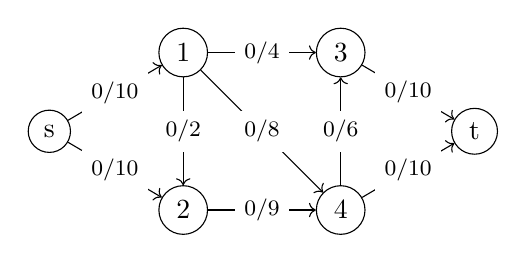
\begin{tikzpicture}[scale=1,every edge quotes/.style={fill=white,font=\footnotesize},every circle node/.style={draw}]
    \node[circle] (s) at (0,0) {s};
    \node[circle] (1) at (1.7,1) {1};
    \node[circle] (2) at (1.7,-1) {2};
    \node[circle] (3) at (3.7,1) {3};
    \node[circle] (4) at (3.7,-1) {4};
    \node[circle] (t) at (5.4,0) {t};
    \draw (s) edge["0/10",->]  (1) ;
    \draw (s) edge["0/10",->]  (2) ;
    \draw (1) edge["0/2",->]  (2) ;
    \draw (1) edge["0/4",->]  (3) ;
    \draw (1) edge["0/8",->]  (4) ;
    \draw (2) edge["0/9",->]  (4) ;
    \draw (4) edge["0/6",->]  (3) ;
    \draw (3) edge["0/10",->]  (t) ;
    \draw (4) edge["0/10",->]  (t) ;    
    \end{tikzpicture}
    &
    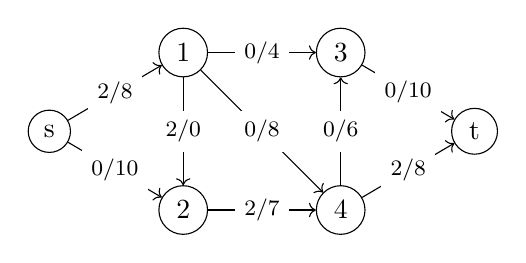
\begin{tikzpicture}[every edge quotes/.style={fill=white,font=\footnotesize},every circle node/.style={draw}]
    \node[circle] (s) at (0,0) {s};
    \node[circle] (1) at (1.7,1) {1};
    \node[circle] (2) at (1.7,-1) {2};
    \node[circle] (3) at (3.7,1) {3};
    \node[circle] (4) at (3.7,-1) {4};
    \node[circle] (t) at (5.4,0) {t};
    \draw (s) edge["2/8",->]  (1) ;
    \draw (s) edge["0/10",->]  (2) ;
    \draw (1) edge["2/0",->]  (2) ;
    \draw (1) edge["0/4",->]  (3) ;
    \draw (1) edge["0/8",->]  (4) ;
    \draw (2) edge["2/7",->]  (4) ;
    \draw (4) edge["0/6",->]  (3) ;
    \draw (3) edge["0/10",->]  (t) ;
    \draw (4) edge["2/8",->]  (t) ;
    \end{tikzpicture}\\
    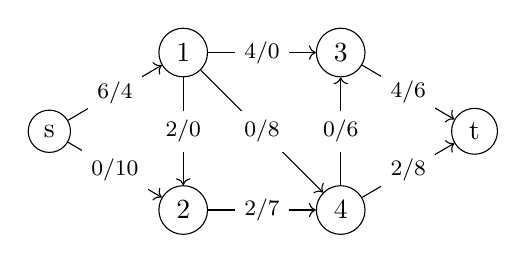
\begin{tikzpicture}[scale=1,every edge quotes/.style={fill=white,font=\footnotesize},every circle node/.style={draw}]
    %13
    \node[circle] (s) at (0,0) {s};
    \node[circle] (1) at (1.7,1) {1};
    \node[circle] (2) at (1.7,-1) {2};
    \node[circle] (3) at (3.7,1) {3};
    \node[circle] (4) at (3.7,-1) {4};
    \node[circle] (t) at (5.4,0) {t};
    \draw (s) edge["6/4",->]  (1) ;
    \draw (s) edge["0/10",->]  (2) ;
    \draw (1) edge["2/0",->]  (2) ;
    \draw (1) edge["4/0",->]  (3) ;
    \draw (1) edge["0/8",->]  (4) ;
    \draw (2) edge["2/7",->]  (4) ;
    \draw (4) edge["0/6",->]  (3) ;
    \draw (3) edge["4/6",->]  (t) ;
    \draw (4) edge["2/8",->]  (t) ; 
    \end{tikzpicture}
    &
    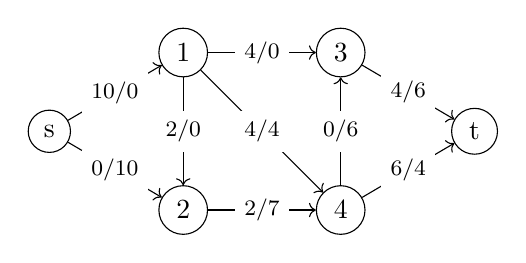
\begin{tikzpicture}[every edge quotes/.style={fill=white,font=\footnotesize},every circle node/.style={draw}]
    %14
    \node[circle] (s) at (0,0) {s};
    \node[circle] (1) at (1.7,1) {1};
    \node[circle] (2) at (1.7,-1) {2};
    \node[circle] (3) at (3.7,1) {3};
    \node[circle] (4) at (3.7,-1) {4};
    \node[circle] (t) at (5.4,0) {t};
    \draw (s) edge["10/0",->]  (1) ;
    \draw (s) edge["0/10",->]  (2) ;
    \draw (1) edge["2/0",->]  (2) ;
    \draw (1) edge["4/0",->]  (3) ;
    \draw (1) edge["4/4",->]  (4) ;
    \draw (2) edge["2/7",->]  (4) ;
    \draw (4) edge["0/6",->]  (3) ;
    \draw (3) edge["4/6",->]  (t) ;
    \draw (4) edge["6/4",->]  (t) ; 
    \end{tikzpicture}\\
    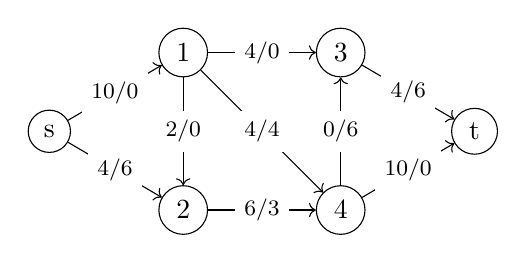
\begin{tikzpicture}[scale=1,every edge quotes/.style={fill=white,font=\footnotesize},every circle node/.style={draw}]
    %24
    \node[circle] (s) at (0,0) {s};
    \node[circle] (1) at (1.7,1) {1};
    \node[circle] (2) at (1.7,-1) {2};
    \node[circle] (3) at (3.7,1) {3};
    \node[circle] (4) at (3.7,-1) {4};
    \node[circle] (t) at (5.4,0) {t};
    \draw (s) edge["10/0",->]  (1) ;
    \draw (s) edge["4/6",->]  (2) ;
    \draw (1) edge["2/0",->]  (2) ;
    \draw (1) edge["4/0",->]  (3) ;
    \draw (1) edge["4/4",->]  (4) ;
    \draw (2) edge["6/3",->]  (4) ;
    \draw (4) edge["0/6",->]  (3) ;
    \draw (3) edge["4/6",->]  (t) ;
    \draw (4) edge["10/0",->]  (t) ;     
    \end{tikzpicture}
    &
    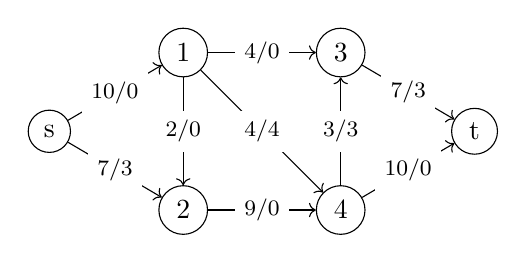
\begin{tikzpicture}[every edge quotes/.style={fill=white,font=\footnotesize},every circle node/.style={draw}]
    %243
    \node[circle] (s) at (0,0) {s};
    \node[circle] (1) at (1.7,1) {1};
    \node[circle] (2) at (1.7,-1) {2};
    \node[circle] (3) at (3.7,1) {3};
    \node[circle] (4) at (3.7,-1) {4};
    \node[circle] (t) at (5.4,0) {t};
    \draw (s) edge["10/0",->]  (1) ;
    \draw (s) edge["7/3",->]  (2) ;
    \draw (1) edge["2/0",->]  (2) ;
    \draw (1) edge["4/0",->]  (3) ;
    \draw (1) edge["4/4",->]  (4) ;
    \draw (2) edge["9/0",->]  (4) ;
    \draw (4) edge["3/3",->]  (3) ;
    \draw (3) edge["7/3",->]  (t) ;
    \draw (4) edge["10/0",->]  (t) ; 
    \end{tikzpicture}\\
\end{tabular}
\end{center}

The path: $s\rightarrow1\rightarrow2\rightarrow4\rightarrow t$,
$s\rightarrow1\rightarrow3\rightarrow t$,
$s\rightarrow1\rightarrow4\rightarrow t$,
$s\rightarrow2\rightarrow4\rightarrow t$,
$s\rightarrow2\rightarrow4\rightarrow3\rightarrow t$.

The edge $a$\tikz{\draw (0,0)edge["c/d",->] (1,0)}$b$ represent an edge from $a$ to $b$ with capacity of $d$, and an edge from $b$ to $a$ with capacity of $c$.

\pagebreak
\section*{Problem 2}
Let $N$ to represent $n$ staff members, $K$ represent $k$ departments, 
$A, B, C, D$ represent four classes.

% \noindent
Create digraph $G=(\{s, t\}\cup A\cup B\cup C,\cup D \cup K \cup N, E)$:
\begin{itemize}
    \item Add source $s$, and unit capacity edges from $s$ to each node in $K$.
    \item Add sink $t$, and $m_1$ capacity edges from $A$ to $t$, $m_2$ capacity edges from $B$ to $t$, $m_3$ capacity edges from $C$ to $t$, $m_4$ capacity edges from $D$ to $t$,
    \item Direct edges from $K_i$ to $N_j$ if $N_j$ belongs to $K_i$ for every $j$, and assign unit capacity.
    \item Direct edges from $N_j$ to $X$ if $N_j$ belongs to $X$($X$ is one of $\{A, B, C, D\}$) for every $j$, and assign unit capacity.
\end{itemize}

Suppose the maximum flow of the network $G$ is $f$, and assume there is a solution to the problem, $H$.
Apply $H$ on $G$ we can get the flow of it is $k$, then we should have $k\leqslant f$. And with $c(\{s\}\cup A\cup B\cup C,\cup D \cup K \cup N, \{t\})=k \geqslant f$, we have $f = k$.

Then use Ford-Fulkerson Algorithm to $G$, we can get $K'$ and  $N'$, 
where every $K_j\in K'$ and every $N_i\in N'$ is on the path.
With $f=k$ and the structure of $G$, we can get $|K'|=|N'|=k$, 
so $N'$ is a set satisfy the requirements of this problem,
every $N_i\in N'$ is the person we need.

\begin{center}
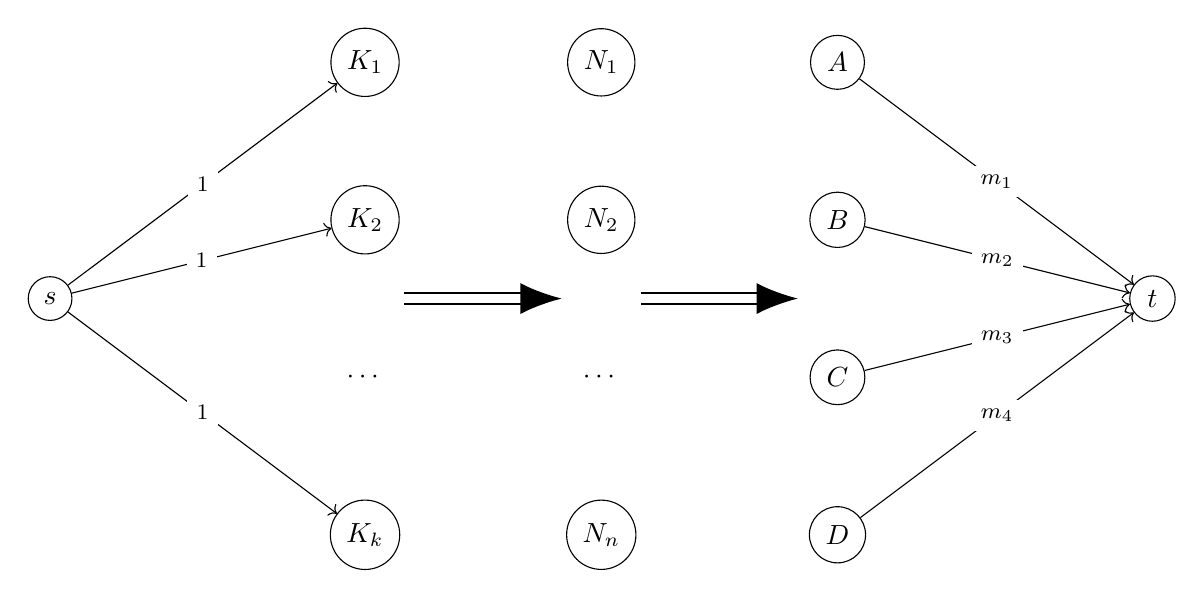
\begin{tikzpicture}[scale=1,every edge quotes/.style={fill=white,font=\footnotesize},every circle node/.style={draw}]
\node[circle] (s) at (0,0) {$s$};
\node[circle] (k1) at (4,3) {$K_1$};
\node[circle] (k2) at (4,1) {$K_2$};
\node (k3) at (4,-1) {$\cdots$};
\node[circle] (k4) at (4,-3) {$K_k$};
\node[circle] (n1) at (7,3) {$N_1$};
\node[circle] (n2) at (7,1) {$N_2$};
\node (n3) at (7,-1) {$\cdots$};
\node[circle] (n4) at (7,-3) {$N_n$};
\node[circle] (a) at (10,3) {$A$};
\node[circle] (b) at (10,1) {$B$};
\node[circle] (c) at (10,-1) {$C$};
\node[circle] (d) at (10,-3) {$D$};
\node[circle] (t) at (14,0) {$t$};
\draw (s) edge["1",->]  (k1) ;
\draw (s) edge["1",->]  (k2) ;
\draw (s) edge["1",->]  (k4) ;
\draw (a) edge["$m_1$",->]  (t) ;
\draw (b) edge["$m_2$",->]  (t) ;
\draw (c) edge["$m_3$",->]  (t) ;
\draw (d) edge["$m_4$",->]  (t) ;
\draw [line width=1pt, double distance=3pt, arrows = {-Latex[length=0pt 3 0]}] (4.5,0) -- (6.5,0);
\draw [line width=1pt, double distance=3pt, arrows = {-Latex[length=0pt 3 0]}] (7.5,0) -- (9.5,0);
\end{tikzpicture}
\end{center}
\pagebreak
\section*{Problem 3}
\begin{enumerate}[(a)]
    \item 
    If there exists a min-cut which edge $(v,u)$ don't cross, then the min-cut will not change, the same with max-flow.
    If edge $(v,u)$ cross a min-cut, the max-flow may increase by $1$.
    
    So we can use BFS to search for if there exists an augmenting path on the residual graph. 
    If there exists an augmenting path, then we can add the path to update max-flow, and increase the value of max-flow by $1$, otherwise the max-flow will stay the same. It will run in $O(|V|+|E|)$.

    \item 
    If we have $c_f(v,u)\geqslant 1$, then nothing change.

    Otherwise, we can use BFS to find a path from $t$ to $s$ on the residual graph. 
    For every edge $(a,b)$(besides $(u,v)$) on the path, decrease $c_f(a,b)$ by $1$, increase $c_f(b,a)$ by $1$.
    And then use BFS to find if there exists an augmenting path from $s$ to $t$.
    If exists, then we can add the path to max-flow, but the value of max-flow will not change; otherwise we should decrease the value of max-flow by $1$.
    It will run in $O(|V|+|E|)$.

\end{enumerate}


\pagebreak
\section*{Problem 4}


\pagebreak
\section*{Problem 5}

Let $N$ to represent $n$ cows, $F$ represent $f$ types of foods, $D$ represent $d$ types of drinks.

Create digraph $G=(\{s, t\}\cup F \cup G \cup N \cup N', E)$:
\begin{itemize}
    \item Add source $s$, and unit capacity edges from $s$ to each node in $F$.
    \item Add sink $t$, and unit capacity edges from each node in $D$ to $t$.
    \item Direct edges from $N_i$ to $N'_i$ for every $i$, and assign unit capacity.
    \item Direct edges from $F_j$ to $N_i$ if food $j$ on the cow $i$'s list, and assign unit capacity.
    \item Direct edges from $N'_i$ to $D_j$ if drink $j$ on the cow $i$'s list, and assign unit capacity.
\end{itemize}

Every path from $s$ to $t$: $s\ra F_j \ra N_i \ra N'_i\ra D_k \ra t$, 
represent a choice that the cow $i$ receives both food $j$ and drink $k$ in his preference lists.
So this problem can convert to find the max-flow of $G$. The set $N'$ is trying to prevent the occurrence of one cow receiving both two types of food and two types of drink at the same time.

Then use Ford-Fulkerson Algorithm to $G$, and find every path: $s\rightarrow F_j\rightarrow N_i\rightarrow N'_i\rightarrow D_k\rightarrow t$, then the set of \{food $j$ and drink $k$ for cow $i$ \} is what we need.

\begin{center}
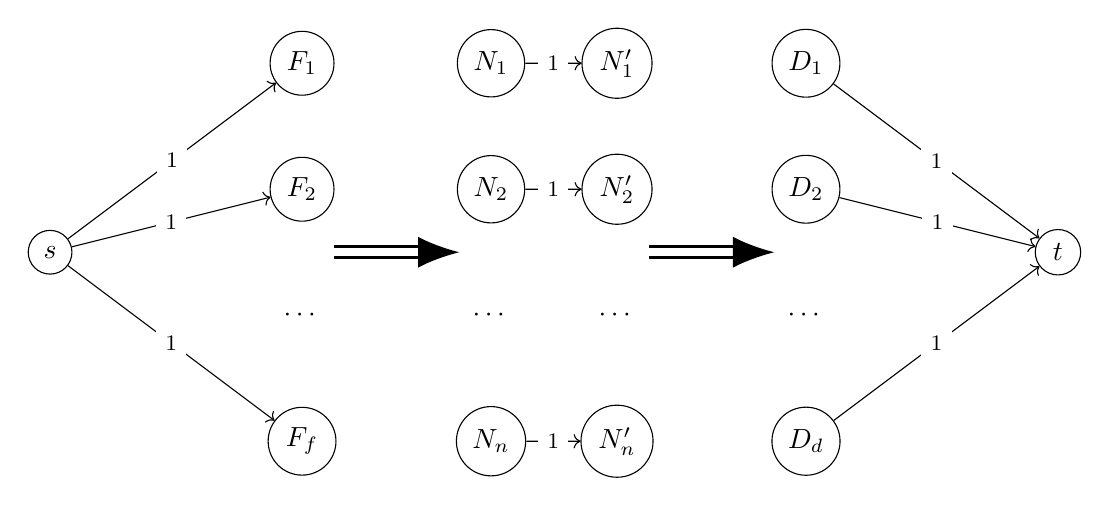
\begin{tikzpicture}[scale=0.8,every edge quotes/.style={fill=white,font=\footnotesize},every circle node/.style={draw}]
    \node[circle] (s) at (0,0) {$s$};
    \node[circle] (f1) at (4,3) {$F_1$};
    \node[circle] (f2) at (4,1) {$F_2$};
    \node (f3) at (4,-1) {$\cdots$};
    \node[circle] (f4) at (4,-3) {$F_f$};
    \node[circle] (n1) at (7,3) {$N_1$};
    \node[circle] (n2) at (7,1) {$N_2$};
    \node (n3) at (7,-1) {$\cdots$};
    \node[circle] (n4) at (7,-3) {$N_n$};
    \node[circle] (n11) at (9,3) {$N'_1$};
    \node[circle] (n22) at (9,1) {$N'_2$};
    \node (n33) at (9,-1) {$\cdots$};
    \node[circle] (n44) at (9,-3) {$N'_n$};
    \node[circle] (d1) at (12,3) {$D_1$};
    \node[circle] (d2) at (12,1) {$D_2$};
    \node (d3) at (12,-1) {$\cdots$};
    \node[circle] (d4) at (12,-3) {$D_d$};
    \node[circle] (t) at (16,0) {$t$};
    \draw (s) edge["1",->]  (f1) ;
    \draw (s) edge["1",->]  (f2) ;
    \draw (s) edge["1",->]  (f4) ;
    \draw (n1) edge["1",->]  (n11) ;
    \draw (n2) edge["1",->]  (n22) ;
    \draw (n4) edge["1",->]  (n44) ;
    \draw (d1) edge["1",->]  (t) ;
    \draw (d2) edge["1",->]  (t) ;
    \draw (d4) edge["1",->]  (t) ;
    \draw [line width=1pt, double distance=3pt, arrows = {-Latex[length=0pt 3 0]}] (4.5,0) -- (6.5,0);
    \draw [line width=1pt, double distance=3pt, arrows = {-Latex[length=0pt 3 0]}] (9.5,0) -- (11.5,0);
    \end{tikzpicture}
\end{center}

\pagebreak
\section*{Problem 6}
Find a min-cut $C$, and the set $E'$, where all edges cross $C$ are in $E'$(Of course, every $e\in E'$ cross $C$).
Then for every $e\in E'$, we can increase $c_f(e)$ by $1$, and then find is there exists an augmenting path on the residual graph(The same as Problem 3(a)).
So if for every $e\in E'$, there don't exist an augmenting path, the $G$ has a unique min-cut, otherwise it hasn't.

For every $e\in E'$, find augmenting path run in $O(|V|+|E|)$, and $|E'|\leqslant |E|$. And finding a min-cut will cost polynomial time.
So this algorithm is a polynomial time algorithm.

\end{document}
